\setcounter{ExampleCounter}{1}
%\marginnote{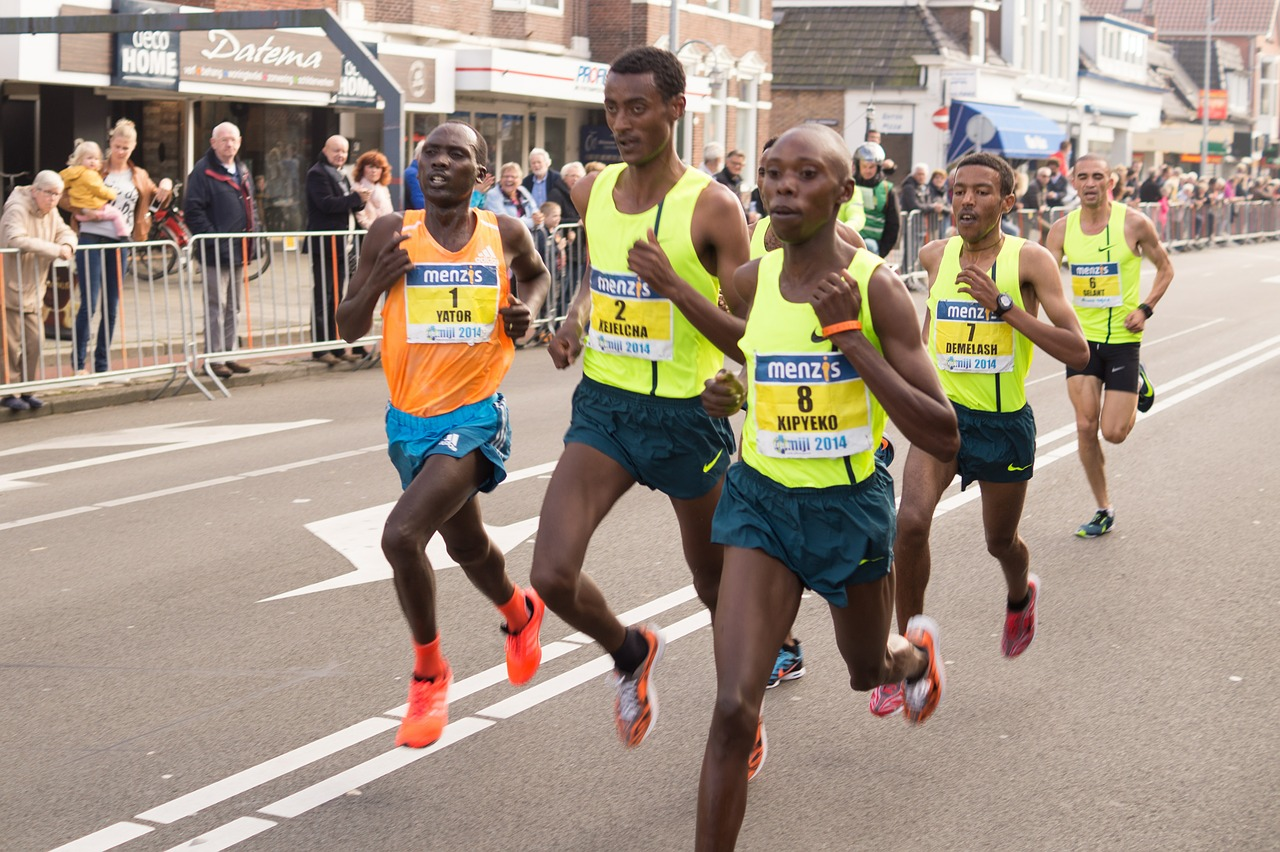
\includegraphics[scale=0.07]{Marathon1}}
If you decide to train for a marathon and you currently run 3 miles a day, you may choose to increase your distance by half a mile every week.  Can we predict how far you'll be running in six weeks, or how long it will take to reach your goal?  With small numbers like these, you could answer those questions without using an equation, but we'll use this as an example to show how to build a simple model from a scenario like this.

\begin{center}
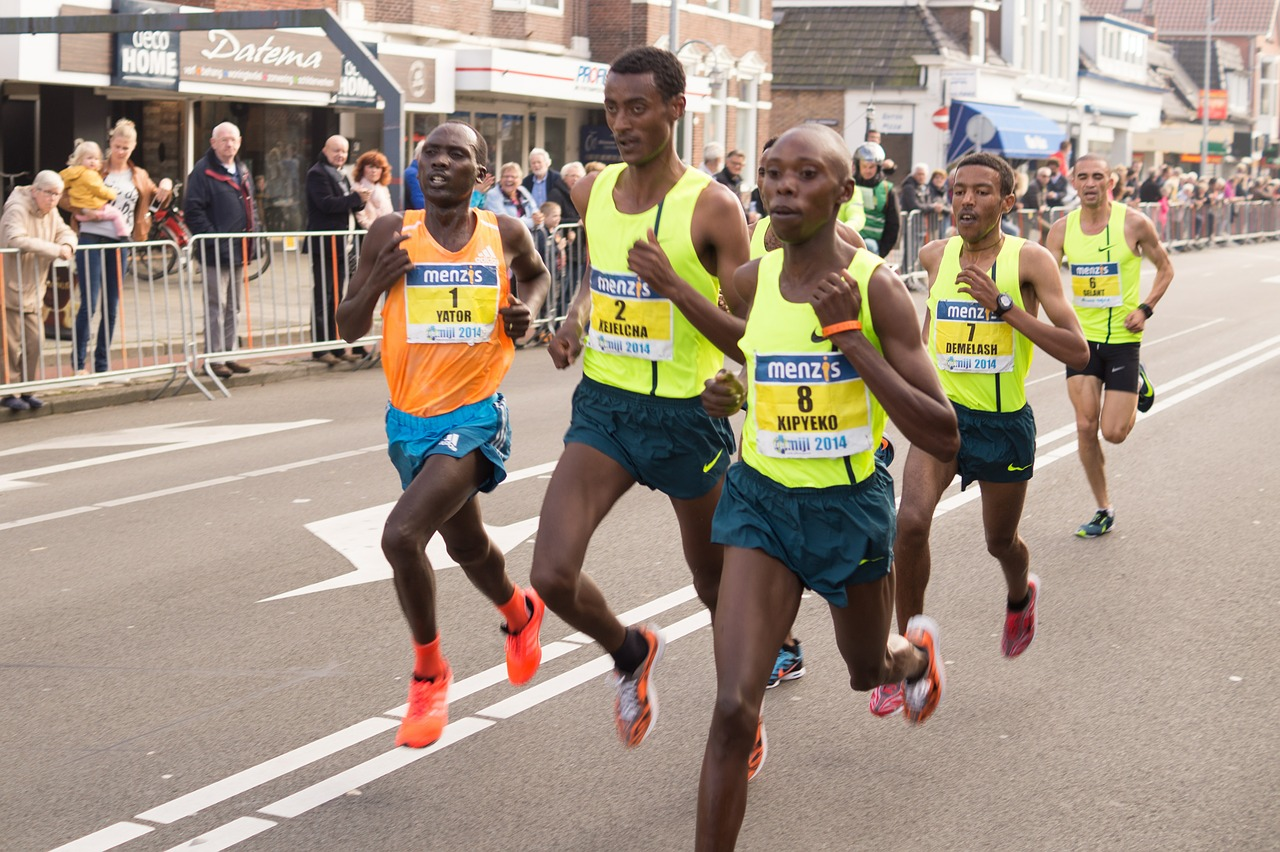
\includegraphics[width=0.8\textwidth]{Marathon1}
\end{center}

Let $P_t$ represent the number of miles that you run after $t$ weeks, so $P_0$ would be the number of miles you currently run, $P_1$ would represent the number of miles you run after 1 week, and so on.  We can define a \textbf{recursive relationship} like the following one to represent the scenario that was laid out.
\begin{align*}
P_0 &= 3\\
P_t &= P_{t-1} + 0.5
\end{align*}

A recursive relationship is one that defines each value in a sequence using previous values.  We could use this relationship to go from $P_0$ to $P_1$ to $P_2$ and so on, all the way to $P_6$ to answer the first question, and we could keep going from one value to the next until we reached 26 to answer the second question.  However, this would be tedious and mindless, so instead we prefer an \textbf{explicit equation}, or closed-form equation.  Especially for predictions far into the future, the recursive form is impractical, even though it arises easily from the problem description.

In this case, the explicit form is pretty straightforward, but deriving it from the recursive form will be instructive:
\begin{align*}
P_0 &= 3\\
P_1 &= 3+0.5\\
P_2 &= 3+0.5+0.5 = 3+(0.5)2\\
P_3 &= 3+0.5+0.5+0.5 = 3 + (0.5)3\\
&\vdots\\
P_t &= 3 + 0.5t
\end{align*}

This explicit equation gives an easy way to quickly answer both questions.  We can substitute 6 for $t$ to find that $P_6 = 3+0.5(6) = 6$ miles, and we can substitute 26 for $P_t$ and solve for $t$ to find how long it'll take to reach your goal:
\begin{align*}
26 &= 3+0.5t\\
23 &= 0.5t\\
46 &= t
\end{align*}
It'll take 46 weeks to reach your goal.
\begin{center}
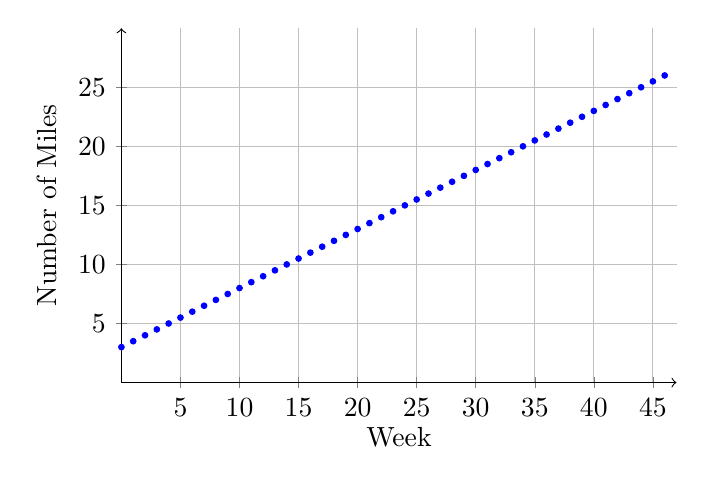
\begin{tikzpicture}
\begin{axis}[
    xmin=0, xmax=47,
    ymin=0, ymax=30,
    axis lines=center,
    axis on top=false,
    domain=0:1,
    x=0.15cm,
    y=0.15cm,
    xtick={5,10,...,45},
    xticklabels={5,10,...,45},
    ytick={0,5,...,25},
    yticklabels={0,5,10,15,20,25,30},
    axis lines=middle,
    axis line style={->},
    x label style={at={(axis description cs:0.5,-0.1)},anchor=north},
    y label style={at={(axis description cs:-0.1,.5)},rotate=90,anchor=south},
    xlabel={Week},
    ylabel={Number of Miles},
    grid=major
    ]
	\addplot [blue,only marks,mark size=1] table {
	0 3
	1 3.5
	2 4
	3 4.5
	4 5
	5 5.5
	6 6
	7 6.5
	8 7
	9 7.5
	10 8
	11 8.5 
	12 9
	13 9.5
	14 10
	15 10.5
	16 11
	17 11.5
	18 12
	19 12.5
	20 13
	21 13.5
	22 14
	23 14.5
	24 15
	25 15.5
	26 16
	27 16.5
	28 17
	29 17.5
	30 18
	31 18.5
	32 19
	33 19.5
	34 20
	35 20.5
	36 21
	37 21.5
	38 22
	39 22.5
	40 23
	41 23.5
	42 24
	43 24.5
	44 25
	45 25.5
	46 26
	};
	%\addplot [blue, thick] table {
	
	%};
\end{axis}
\end{tikzpicture}
\end{center}

This graph shows why we call this \textit{linear} growth.  If we graph the number of miles versus the week, the points lie along a straight line.  This is consistent for every problem where a number grows by a constant amount every time period.  That's the key to linear growth: there's a constant growth amount, which we'll call $d$ (for \emph{difference}), that is added at each step.  For instance, in the marathon example, $d=0.5$ because half a mile is added each week.  Knowing that, the following formula should look familiar, because it is the same form that we developed above.

\begin{formula}{Linear Growth}
If some quantity starts at size $P_0$ and grows by $d$ every time period, then the quantity after $t$ time periods can be predicted using the following formula.

{\Large \[P_t = P_0 + dt\]}

Here $d$ represents the common difference---the amount that the quantity changes each time $t$ increases by 1.\\

Notice that this could refer to linear growth or linear decay; if $d$ is negative, the quantity will decrease linearly.
\end{formula}

Knowing that the key to linear growth is this common difference between terms, we can recognize linear growth from data if each term is the previous term plus a constant.
\begin{center}
\begin{tabular}{p{0.5in} p{0.75in} p{1.25in}}
\textbf{Term} & \textbf{Quantity} & \textbf{Difference from Previous Term}\\
\hline
& & \\
0 & 15 & \\
1 & 27 & 12\\
2 & 39 & 12\\
3 & 51 & 12\\
4 & 63 & 12\\
5 & 75 & 12\\
\end{tabular}
\end{center}
As we can observe in this table, if we note that the quantity adds a constant amount each time, we know that the growth is linear, and we can write the closed-form equation given above.\\

Notice that this is exactly the standard linear equation that you've seen in your algebra classes:
\begin{align*}
y &= mx+b\\
P_t &= dt + P_0
\end{align*}
Here, $P_0$ is the $y$-intercept, since it is the starting point, and thus the value when $t=0$.  Also, $d$ is the slope here, or the amount by which the quantity changes when $t$ increases by 1.

These two equations are the same, but as you'll see when modeling, we often rename the pieces to more closely match the names of the real-world quantities we're measuring.
\pagebreak

\begin{example}[https://www.youtube.com/watch?v=cpaNK4jbMkA&list=PLfmpjsIzhztutjEb8Pg5OBOlI1p80yVoy&index=1]{Elk Population}
The population of elk in a national forest was measured to be 12,000 in 2011 and 15,000 in 2015.  If the population continues to grow linearly at this rate, what do we expect the elk population to be in 2022?

\solline
\marginnote{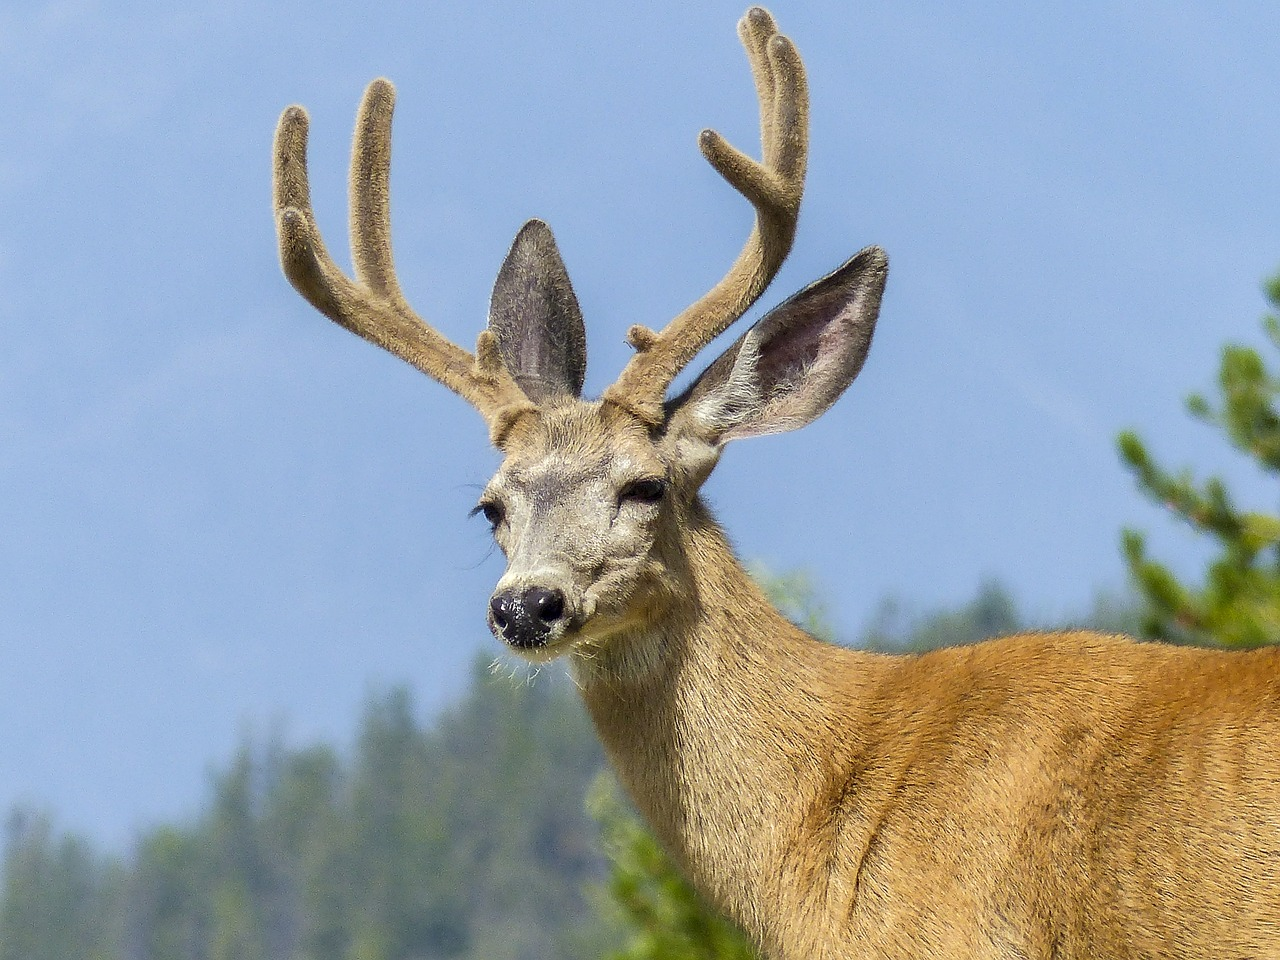
\includegraphics[scale=0.07]{Elk1}}
We first need to define the parts of our linear growth equation.  The initial amount $P_0$ is the amount when $t=0$, but we won't use the actual year 0 as our starting point.  Instead, the initial amount in this problem is given in 2011, so we'll define $t=0$ to be the year 2011, so $P_0=12,000$.\\

Next we need to find $d$, the growth per time period.  Since the time period in this example is one year, we'll need to find how much the population grew each year.
\begin{center}
\begin{tabular}{c c}
\textbf{Year} & \textbf{Population}\\
\hline
0 & 12,000\\
4 & 15,000
\end{tabular}
\end{center}
Since the population grew by 3,000 in 4 years, this represents a growth of 3,000/4 = 750 per year.  Thus $d=750$.\\

Note that this is equivalent to using the slope formula: $\dfrac{\textrm{rise}}{\textrm{run}}$
\begin{align*}
d &= \textrm{ slope }\\
&= \dfrac{\textrm{change in population}}{\textrm{change in time}}\\
&= \dfrac{15,000 - 12,000}{2015 - 2011}\\
&= \dfrac{3000}{4}\\
&= 750
\end{align*}

Now we can write the explicit equation that models this population growth:
\[P_t = 12,000 + 750t\]

To answer the question, we note that 2022 corresponds to $t=11$, since 2022 is 11 years after 2011.
\begin{align*}
P_{11} &= 12,000 + 750(11)\\
&= \boxed{20,250 \textrm{ elk}}
\end{align*}
\end{example}

\begin{try}[http://hartleymath.com/versatilemath/tryit/\#/growth-models--linear-growth-model-(trout-population)]
If we estimated the population of trout in a pond to be 2200 in 2008 and 3500 in 2012, construct a linear model to predict the population in 2017.
\end{try}

Notice the key to that last problem: by knowing the population at the beginning and at the end, we can how much the population changes in a single year by dividing the total change by the number of years that elapsed.

In the next example, we'll look at data that is nearly linear, but not exactly.  However, for the purposes of making predictions, we'll treat it as if it follows a linear trend (remember, in the real world, data is messy).  We'll do exactly the same thing we just did in the previous example; we'll simply focus on the amount at the beginning and at the end, and divide the total growth by the amount of time that passed.
\vfill
\pagebreak

\begin{example}[https://www.youtube.com/watch?v=QoOdfeLBN0o&list=PLfmpjsIzhztutjEb8Pg5OBOlI1p80yVoy&index=2]{Gasoline Consumption}
Gasoline consumption in the US has been increasing steadily.  Data from 1995 to 2004 is shown below.  Find a linear model for this data, and use it to predict consumption in 2018.  If the trend continues, when will consumption reach 200 billion gallons?

\solline
\marginnote{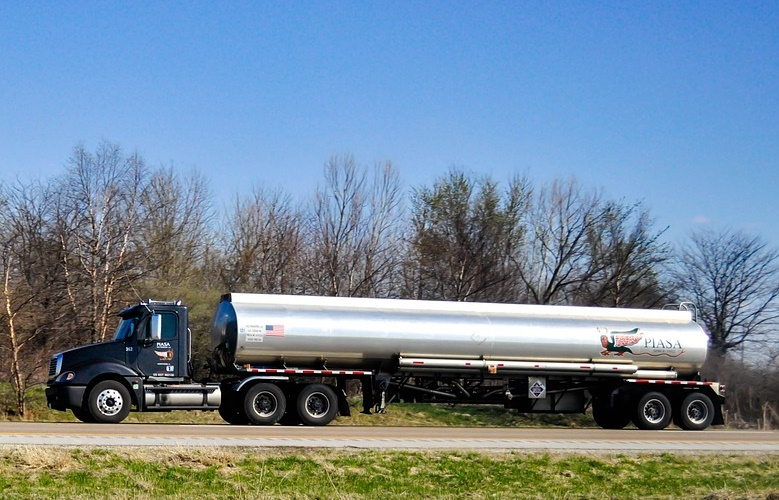
\includegraphics[scale=0.16]{GasTanker1}}
\begin{center}
\begin{tabular}{|p{1in} | c | c | c | c | c | c | c | c | c | c|}
\hline
\textbf{Year} & '95 & '96 & '97 & '98 & '99 & '00 & '01 & '02 & '03 & '04\\
\hline
\parbox{0.9in}{\textbf{Consumption (billions}\\ \textbf{of gallons)}} & 116 & 118 & 119 & 123 & 125 & 126 & 128 & 131 & 133 & 136\\
\hline
\end{tabular}
\end{center}

If we plot this data, it appears to have an approximately linear relationship.
\begin{center}
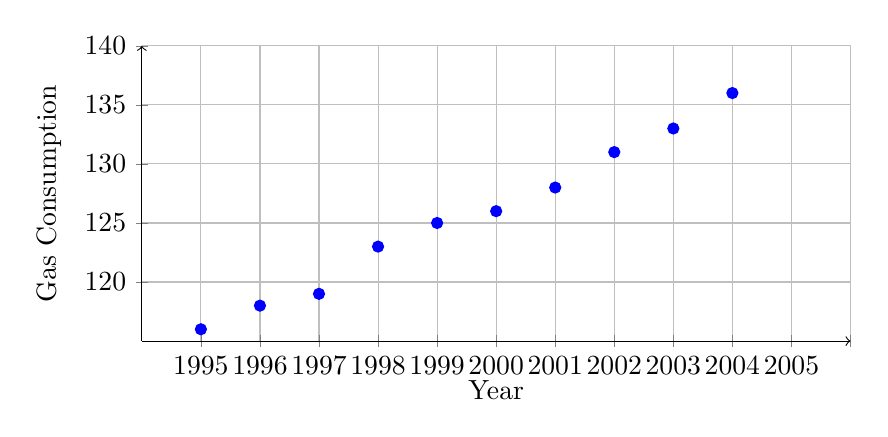
\begin{tikzpicture}
\begin{axis}[
    xmin=0, xmax=12,
    ymin=0, ymax=25,
    axis lines=center,
    axis on top=false,
    domain=0:1,
    x=0.75cm,
    y=0.15cm,
    xtick={0,1,...,12},
    xticklabels={1994,1995,1996,1997,1998,1999,2000,2001,2002,2003,2004,2005},
    ytick={0,5,...,25},
    yticklabels={115,120,125,130,135,140},
    axis lines=middle,
    axis line style={->},
    x label style={at={(axis description cs:0.5,-0.1)},anchor=north},
    y label style={at={(axis description cs:-0.1,.5)},rotate=90,anchor=south},
    xlabel={Year},
    ylabel={Gas Consumption},
    grid=major
    ]
	\addplot [blue,only marks] table {
	1 1
	2 3
	3 4
	4 8
	5 10
	6 11
	7 13
	8 16
	9 18
	10 21
	};
	%\addplot [blue, thick] table {
	
	%};
\end{axis}
\end{tikzpicture}
\end{center}

One way to find a linear trend for data like this is a statistical technique known as \textit{linear regression}.  We will see examples of how to use the calculator for regression later in this section, and the chapter on Statistics will describe linear regression in more detail.

For now, though, we'll simply use the data from the first and last years to find the average growth each year (the slope of the line).\marginnote{We could use the data from any two years to calculate the slope (and we would get slightly different answers), but a common convention is to use the first and last years.  You should follow this convention when answering the homework questions.}
\begin{center}
\begin{tabular}{c | c}
\textbf{Year} & \textbf{Consumption}\\
\hline
1995 & 116\\
2004 & 136
\end{tabular}
\end{center}

\begin{align*}
d &= \textrm{ slope } = \dfrac{\textrm{change in consumption}}{\textrm{change in time}} = \dfrac{136 - 116}{2004 - 1995} = \dfrac{20}{9}\\
&= 2.22 \textrm{ billion gallons per year}
\end{align*}

Now we can write our model (in billions of gallons):
\[\boxed{P_t = 116 + 2.2t}\]
\begin{center}
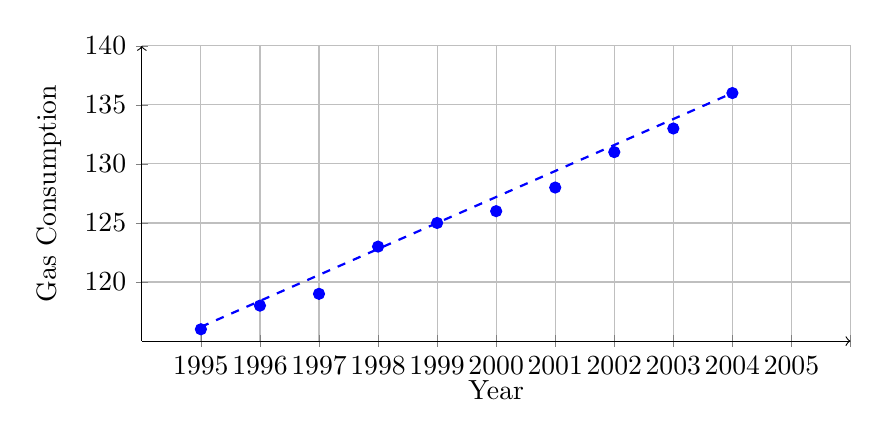
\begin{tikzpicture}
\begin{axis}[
    xmin=0, xmax=12,
    ymin=0, ymax=25,
    axis lines=center,
    axis on top=false,
    domain=0:1,
    x=0.75cm,
    y=0.15cm,
    xtick={0,1,...,12},
    xticklabels={1994,1995,1996,1997,1998,1999,2000,2001,2002,2003,2004,2005},
    ytick={0,5,...,25},
    yticklabels={115,120,125,130,135,140},
    axis lines=middle,
    axis line style={->},
    x label style={at={(axis description cs:0.5,-0.1)},anchor=north},
    y label style={at={(axis description cs:-0.1,.5)},rotate=90,anchor=south},
    xlabel={Year},
    ylabel={Gas Consumption},
    grid=major
    ]
	\addplot [blue,only marks] table {
	1 1
	2 3
	3 4
	4 8
	5 10
	6 11
	7 13
	8 16
	9 18
	10 21
	};
	\addplot [blue, thick,dashed,domain=1:10] {2.2*x-1};
\end{axis}
\end{tikzpicture}
\end{center}
\vfill
\pagebreak

We can use our model to make predictions about the future, using the simplifying assumption that the previous trend continues unchanged.
\begin{itemize}
\item Predicting gas consumption in 2018, when $t=23$:\marginnote{This example illustrates the two main types of questions that we often want to answer:\\ \text{}\\
1. Predicting the value of what we are measuring at a given point in time.\\ \text{}\\
2. Predicting the point in time when the thing we are measuring will reach a certain value.}
\[P_{23} = 116 + 2.2(23) = \boxed{166.6}\]
Our model predicts that the US will consume 166.6 billion gallons of gasoline in 2018 if the current trend continues.

\item Predicting when consumption reaches 200 billion gallons:
\begin{align*}
200 &= 116 + 2.2t\\
84 &= 2.2t\\
\boxed{38.18} &= t
\end{align*}
This model predicts that gas consumption will reach 200 billion gallons about 38 years after 1995, or the year 2033.
\end{itemize}
\end{example}

\begin{try}[http://hartleymath.com/versatilemath/tryit/\#/growth-models--stay-at-home-fathers]
The number of stay-at-home fathers in Canada has been growing steadily at an approximately linear rate.  Use the data from the table below to find an explicit formula for the number of stay-at-home fathers and use it to predict the number in 2020.  Use 1976 and 2010 to find the average rate of change.
\begin{center}
\begin{tabular}{|p{1.25in} | c | c | c | c | c|}
\hline
\textbf{Year} & 1976 & 1984 & 1991 & 2000 & 2010\\
\hline
\textbf{Number of stay-at-home fathers} & 20,610 & 28,725 & 43,530 & 47,665 & 53,555\\
\hline
\end{tabular}
\end{center}
\end{try}

Again, we understand that this model is not perfect; the US will most likely not consume exactly 166.6 billion gallons of gas in 2018, but we expect consumption to be \textit{about} that.  In practice, we'll often make predictions and then compare them to actual measured results to assess the accuracy of our model.  A very simple linear model like this will likely have fairly large error; more sophisticated models tend to have smaller errors.

\subsection{Predicting Time}
As we pointed out in the previous example, there are generally two questions that we'll encounter with mathematical models like the ones in this chapter:
\begin{itemize}
\item At a given time, find the amount
\item For a given amount, find the time it will take to reach that level
\end{itemize}

The first question is generally easier, simply because of how the formula is arranged:
\[P_t = P_0 + dt\]
Since we know everything on the right-hand side of the equation in this case, we can plug it all in and simply carry out the arithmetic; what we want to know is already isolated on the left side.

It's slightly more tricky to solve for $t$ in the second question, because it requires some algebra to rearrange the pieces of the formula so that $t$ will be isolated on one side.  This gets even more difficult for more complicated models, like the ones in the rest of the chapter, because the algebraic steps are more involved.

\subsubsection*{Another option: use a calculator}
Although you should be able to carry out the algebraic steps, and it will likely be quicker to do so with linear models, let's see how to use the calculator to accomplish the same purpose.  What we're about to see will work no matter which part of the equation we want to solve for, so we will return to this method in each section in this chapter when we want to solve for $t$.
\vfill
\pagebreak

The key to this method involves graphing both sides of an equation and using the \texttt{intersect} option on a graphing calculator.  If you have a TI-83 or 84 or similar, you can look under the \texttt{CALC} menu, which you can find by pressing \calcbutton{2ND} and \calcbutton{TRACE}:
\begin{center}
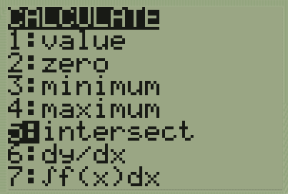
\includegraphics[width=2in]{calculatorIntersect}
\end{center}

Before diving into the details, let's see why this works by going all the way back to the opening example of this section: the marathon training program.  Remember that we drew this graph to represent the number of miles that you would run each week:
\begin{center}
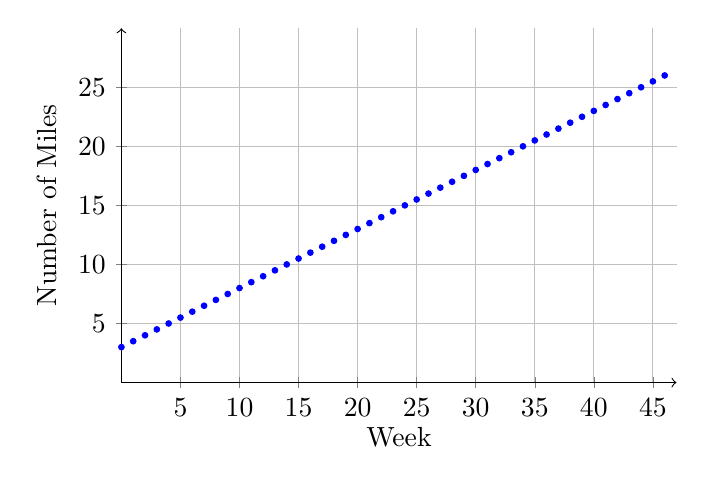
\begin{tikzpicture}
\begin{axis}[
    xmin=0, xmax=47,
    ymin=0, ymax=30,
    axis lines=center,
    axis on top=false,
    domain=0:1,
    x=0.15cm,
    y=0.15cm,
    xtick={5,10,...,45},
    xticklabels={5,10,...,45},
    ytick={0,5,...,25},
    yticklabels={0,5,10,15,20,25,30},
    axis lines=middle,
    axis line style={->},
    x label style={at={(axis description cs:0.5,-0.1)},anchor=north},
    y label style={at={(axis description cs:-0.1,.5)},rotate=90,anchor=south},
    xlabel={Week},
    ylabel={Number of Miles},
    grid=major
    ]
	\addplot [blue,only marks,mark size=1] table {
	0 3
	1 3.5
	2 4
	3 4.5
	4 5
	5 5.5
	6 6
	7 6.5
	8 7
	9 7.5
	10 8
	11 8.5 
	12 9
	13 9.5
	14 10
	15 10.5
	16 11
	17 11.5
	18 12
	19 12.5
	20 13
	21 13.5
	22 14
	23 14.5
	24 15
	25 15.5
	26 16
	27 16.5
	28 17
	29 17.5
	30 18
	31 18.5
	32 19
	33 19.5
	34 20
	35 20.5
	36 21
	37 21.5
	38 22
	39 22.5
	40 23
	41 23.5
	42 24
	43 24.5
	44 25
	45 25.5
	46 26
	};
	%\addplot [blue, thick] table {
	
	%};
\end{axis}
\end{tikzpicture}
\end{center}

Now, let's ask this question: how long will it take to reach the goal of running 26 miles?  Notice that what this means on the graph is: when does that blue line reach a height of 26?  If we draw a horizontal line at 26, we can zero in on the point where the two lines cross (or intersect) and trace downward to the $x$-axis to find the time when that intersection occurs.

\begin{center}
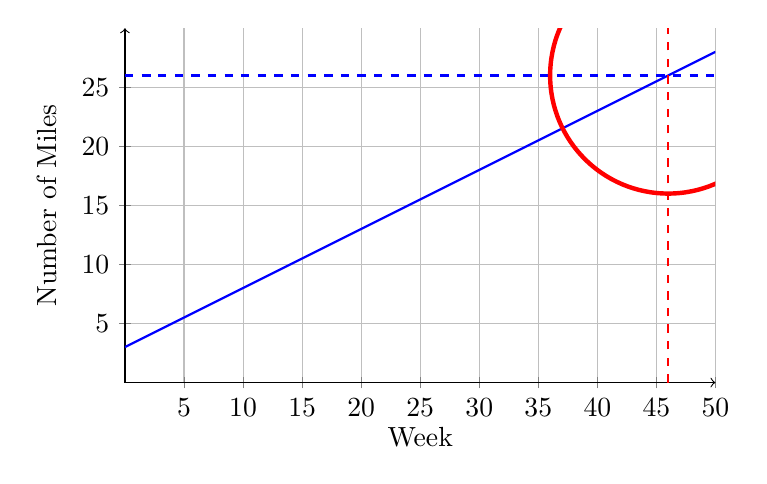
\begin{tikzpicture}
\begin{axis}[
    xmin=0, xmax=50,
    ymin=0, ymax=30,
    axis lines=center,
    axis on top=false,
    domain=0:1,
    x=0.15cm,
    y=0.15cm,
    xtick={5,10,...,50},
    xticklabels={5,10,...,50},
    ytick={0,5,...,25},
    yticklabels={0,5,10,15,20,25,30},
    axis lines=middle,
    axis line style={->},
    x label style={at={(axis description cs:0.5,-0.1)},anchor=north},
    y label style={at={(axis description cs:-0.1,.5)},rotate=90,anchor=south},
    xlabel={Week},
    ylabel={Number of Miles},
    grid=major
    ]
	\addplot [blue, thick,domain=0:50] {0.5*x+3};
	\addplot [blue, thick,dashed,domain=0:50] {26};
	\draw [red, thick, dashed] (axis cs:46,0) -- (axis cs:46,30);
	\draw [red, ultra thick] (axis cs:46,26) circle (10);
\end{axis}
\end{tikzpicture}
\end{center}

In other words, when we find the coordinates of the intersection point, the $y$-coordinate will be the level we're given to predict the time for, and the $x$-coordinate will be the time at which that level is reached.\\

On the calculator, this means we have to graph two functions: one will be the model that we have built ($P_t = P_0 + dt$ for linear models in this section, other formulas for later sections), and the other will be a constant value, whatever value we want to know the corresponding time for.  Once we find the intersection, the $x$-coordinate will be the time value that we're looking for.

To illustrate how to use this method, we'll continue to use the same example: remember that the model we built was $P_t = 3 + 0.5t$, and we wanted to predict when the number of miles would reach 26.  Thus, we need to graph $y_1=3+0.5x$ and $y_2=26$ on the calculator; note that the calculator always uses $x$ and $y$ instead of $t$ and $P_t$.
\vfill
\pagebreak

\subsubsection*{Step 1: graph both functions}
To begin, press the \calcbutton{Y=} button in the upper-left corner to open the graphing menu, then enter the two functions as $Y_1$ and $Y_2$.  Note that to enter $X$, use the button labeled $\boxed{X, T, \theta, n}$
\begin{center}
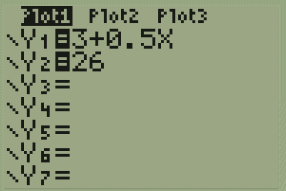
\includegraphics[width=2in]{calculatorIntersectEx1}
\end{center}

\subsubsection*{Step 2: zoom to see the intersection}
When you press \calcbutton{GRAPH} you may see something like this:
\begin{center}
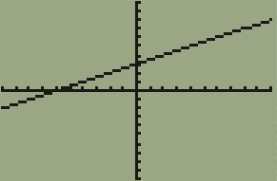
\includegraphics[width=2in]{calculatorIntersectEx2}
\end{center}

Only one line is visible, because the window is too zoomed in to see the other.  To zoom out, you can press the \calcbutton{ZOOM} button and select one of the options, like \texttt{3. Zoom Out}.  If you press the \calcbutton{WINDOW} button, though, you can manually set the boundaries of the window, and if you have a sense of roughly where the intersection should occur, that's usually the easiest way to adjust the view so that you can see both lines.

In this case, we know that the upper end of the window needs to go up to at least 26, since that is the $y$-coordinate of the intersection, so let's use 30 as the upper limit.  With a bit of trial and error, we can find a reasonable upper limit on $x$ as well; we'll use 50 for this one.
\begin{center}
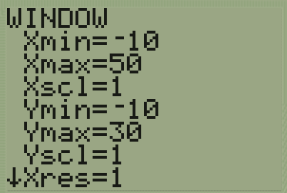
\includegraphics[width=2in]{calculatorIntersectEx3}
\end{center}

If you press \calcbutton{GRAPH} again, you should see this:
\begin{center}
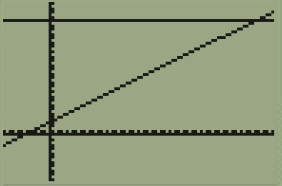
\includegraphics[width=2in]{calculatorIntersectEx4}
\end{center}

We can now see the intersection point on the graph, but we have a bit more work to do to find its coordinates.
\pagebreak

\subsubsection*{Step 3: find the intersection}
Now if you press \calcbutton{2ND} and \calcbutton{TRACE} to open the \texttt{CALC} menu and select the option labeled \texttt{5. intersect}, you'll see something like this:
\begin{center}
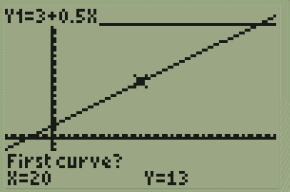
\includegraphics[width=2in]{calculatorIntersectEx5}
\end{center}

What's happening here?  Without getting too specific, the way the calculator finds the intersection point involves starting with an initial guess, and then searching nearby in both directions to find the crossing point.  This means it will ask where you want to start looking on the first curve, where you want to start looking on the second curve, and where your overall initial guess is.  You can use the arrow keys to move the blinking cursor closer to the intersection if you like, but for simple examples like the ones in this chapter, the calculator will find it even if we don't feed it a starting point that is close by.

In practice, this means that if you like, you can simple press \calcbutton{ENTER} three times to accept the default starting values.

Once you do this, you should see the following:
\begin{center}
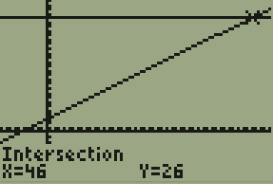
\includegraphics[width=2in]{calculatorIntersectEx6}
\end{center}

At the bottom of the screen, you can see the coordinates of the intersection point.  Notice that the $y$-coordinate is no surprise; that's based on the given number of miles that we were trying to reach.  The $x$-coordinate is the answer we were looking for, the value of $t$ when we reach 26 miles.

\subsection{Linear Regression Using the Calculator}
Usually when we build a model, we do so using data from the past to predict the future.  In most of the examples in this section, we drew a straight line by selecting the first and last points and finding the slope that connected them.

There is another approach, using a statistical technique known as \textbf{linear regression}.  We will omit the details here, but a more thorough discussion can be found in the Statistics chapter.  For our purposes, we will simply see how to use a graphing calculator to find the equation of a line that most closely fits the data we're given.

Rather than simply using two points, linear regression takes all of the data points into account and builds a \textit{line of best fit}; the principles needed to describe how this best-fit process works require some statistics knowledge, so we will not discuss it further in this chapter.\\

We'll use the gasoline consumption example to show how to use the calculator for this.  Recall that we were given the following data (and the resulting graph):
\begin{center}
\begin{tabular}{|p{1in} | c | c | c | c | c | c | c | c | c | c|}
\hline
\textbf{Year} & '95 & '96 & '97 & '98 & '99 & '00 & '01 & '02 & '03 & '04\\
\hline
\parbox{0.9in}{\textbf{Consumption (billions}\\ \textbf{of gallons)}} & 116 & 118 & 119 & 123 & 125 & 126 & 128 & 131 & 133 & 136\\
\hline
\end{tabular}
\end{center}

\begin{center}
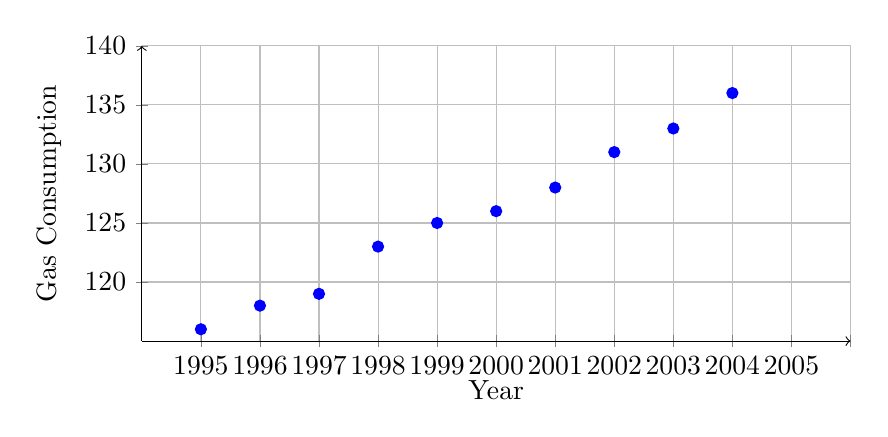
\begin{tikzpicture}
\begin{axis}[
    xmin=0, xmax=12,
    ymin=0, ymax=25,
    axis lines=center,
    axis on top=false,
    domain=0:1,
    x=0.75cm,
    y=0.15cm,
    xtick={0,1,...,12},
    xticklabels={1994,1995,1996,1997,1998,1999,2000,2001,2002,2003,2004,2005},
    ytick={0,5,...,25},
    yticklabels={115,120,125,130,135,140},
    axis lines=middle,
    axis line style={->},
    x label style={at={(axis description cs:0.5,-0.1)},anchor=north},
    y label style={at={(axis description cs:-0.1,.5)},rotate=90,anchor=south},
    xlabel={Year},
    ylabel={Gas Consumption},
    grid=major
    ]
	\addplot [blue,only marks] table {
	1 1
	2 3
	3 4
	4 8
	5 10
	6 11
	7 13
	8 16
	9 18
	10 21
	};
	%\addplot [blue, thick] table {
	
	%};
\end{axis}
\end{tikzpicture}
\end{center}

The model we built in that example was $P_t = 116 + 2.2t$; we'll keep this handy to compare it to the answer we get using regression.

\subsubsection*{Step 1: enter the data}
First, we need to enter the data that we're given (in full).  To do this, press the \calcbutton{STAT} button; the first menu that you will see should look like this:
\begin{center}
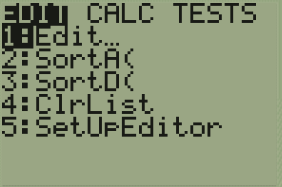
\includegraphics[width=2in]{gmRegression1}
\end{center}

Simply press \calcbutton{ENTER} to enter the \texttt{Edit} menu, where we can enter the data; first, you should see the following (if there is data already there, simply use the arrow keys to move up to the label of one of the lists, and press \calcbutton{CLEAR}):

\begin{center}
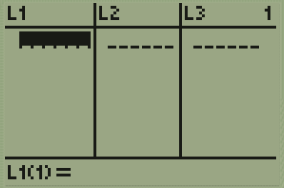
\includegraphics[width=2in]{gmRegression2}
\end{center}

In list \texttt{L1}, enter the values for $t$.  Notice that here we set 1995 as the initial year, or year 0, so start with 0 and enter enough values to get to 2004 (year 9).  In list \texttt{L2}, enter the values for gasoline consumption.

\begin{center}
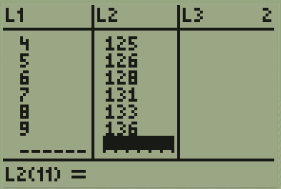
\includegraphics[width=2in]{gmRegression3}
\end{center}
\pagebreak

\subsubsection*{Step 2: calculate the regression equation}

Now, to calculate the regression equation, press the \calcbutton{STAT} button again, and use the right arrow key to move to the \texttt{CALC} menu.  There are many options here, but the one we want at the moment is \texttt{4: LinReg(ax+b)}.  Notice that this means that we'll receive answers for \texttt{a} and \texttt{b}, and these will represent the slope and intercept, respectively.

\begin{center}
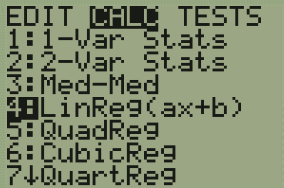
\includegraphics[width=2in]{gmRegression4}
\end{center}

If you select the linear regression option, you should see the following menu:

\begin{center}
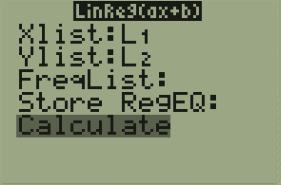
\includegraphics[width=2in]{gmRegression5}
\end{center}

Since we entered the time values in \texttt{L1} and the consumption values in \texttt{L2}, we don't need to change anything here, so simply scroll down to select \texttt{Calculate} and press \calcbutton{ENTER}\ , which shows the results:

\begin{center}
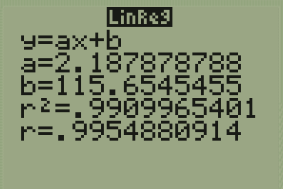
\includegraphics[width=2in]{gmRegression6}
\end{center}

For now, all we're interested in is the values of \texttt{a} and \texttt{b}; to put it in more familiar terms, the equation of the regression model is
\[P_t = 115.7 + 2.19t\]

Compare this to the one we built by hand.  Since this data was fairly linear, there isn't much difference between the two answers; if there were \emph{outliers} (unusual values that deviate significantly from the linear trend), there might be a greater difference.

In general, the manual method is easier and quicker to do, but this statistical method gives more accurate results.
\pagebreak

\subsection{Using Excel}
We can also use Excel to calculate regression equations.  To begin, enter the data as shown (we're using the same example as we did with the calculator, for comparison):

\begin{center}
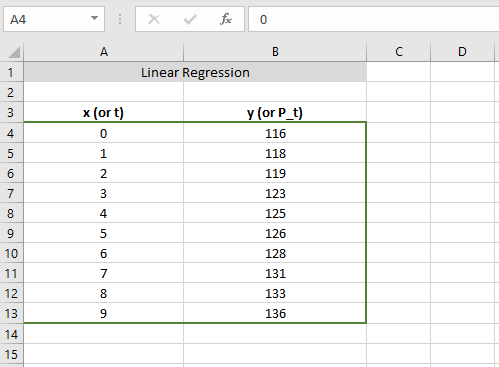
\includegraphics[width=0.6\textwidth]{gmRegressionExcel1}
\end{center}

Next, we need to insert a scatterplot of these data points; select the Insert menu at the top of the screen, then select the scatterplot option under the Charts section (select the first type of scatterplot under that submenu).

\begin{center}
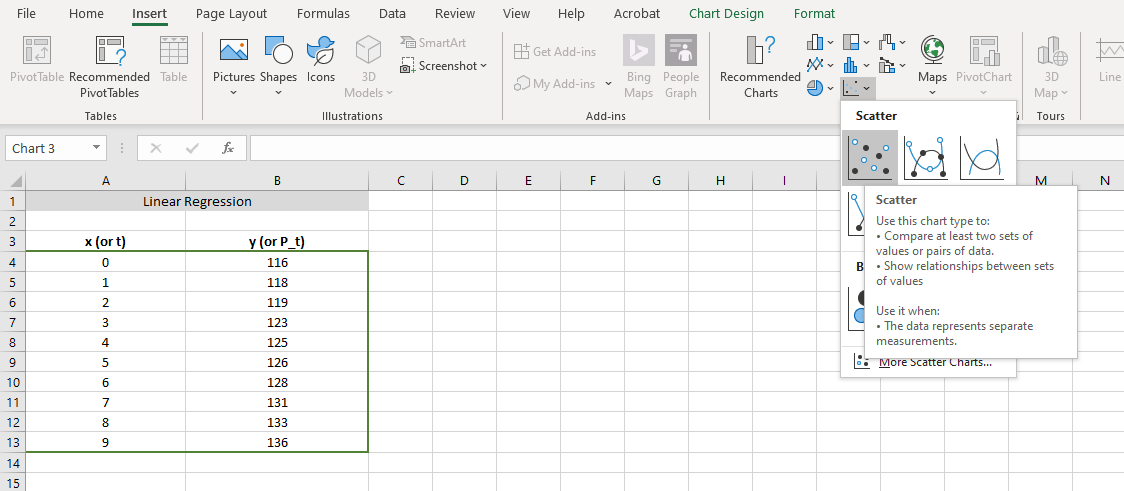
\includegraphics[width=0.6\textwidth]{gmRegressionExcel2}
\end{center}

This creates a graph similar to the one that we drew earlier for this same example; we could add a title to the chart and the axes, but we won't bother for this example.

\begin{center}
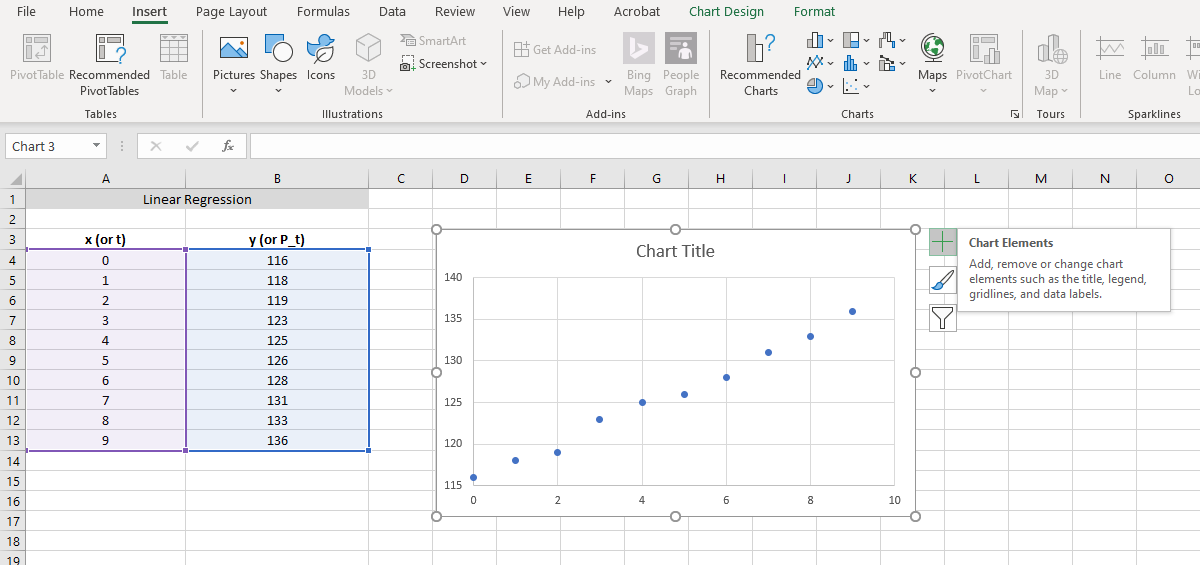
\includegraphics[width=0.6\textwidth]{gmRegressionExcel3}
\end{center}

To add a regression line, click on the plus symbol at the upper right (when the chart is selected).  One of the options is to add a trendline.  If you check that box, the line will be drawn, but by default, Excel won't show the equation of the line, which is what we're after, so we need to select ``More Options'' after clicking on the arrow next to the trendline option.

\begin{center}
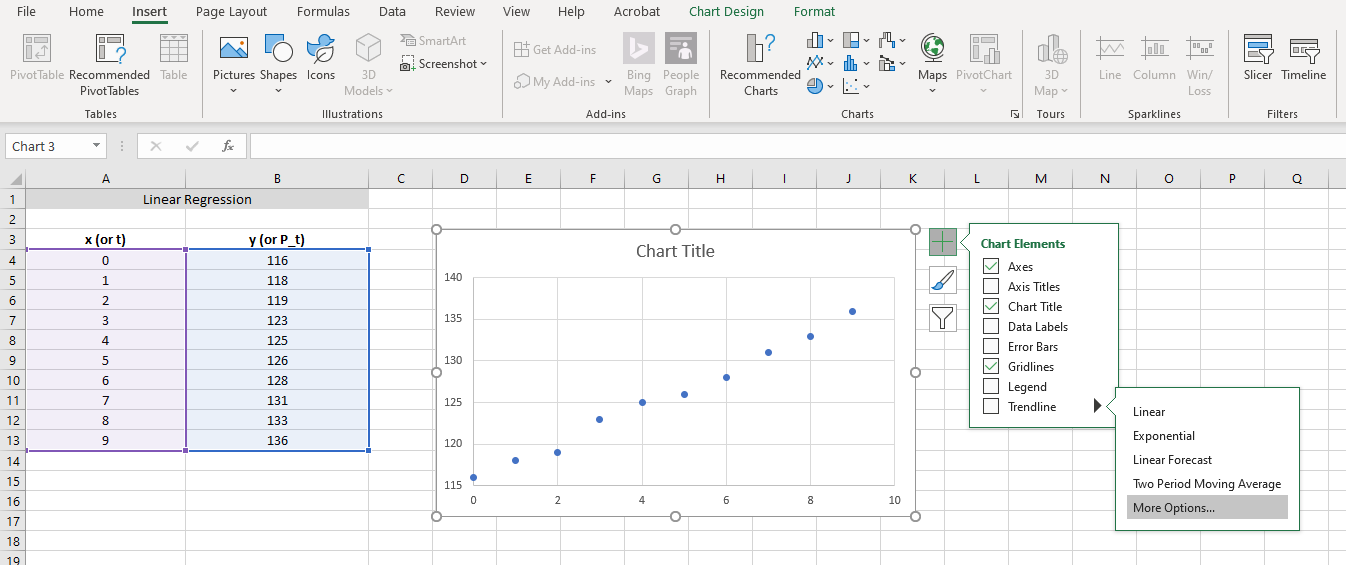
\includegraphics[width=0.6\textwidth]{gmRegressionExcel4}
\end{center}

This brings up the following menu.  Notice that there are different types of equations we can use to model the data, including several that we'll encounter later in the chapter.  For now, though, leave the linear option selected, but check the box at the bottom of the menu that says ``Display Equation on chart.''

\begin{center}
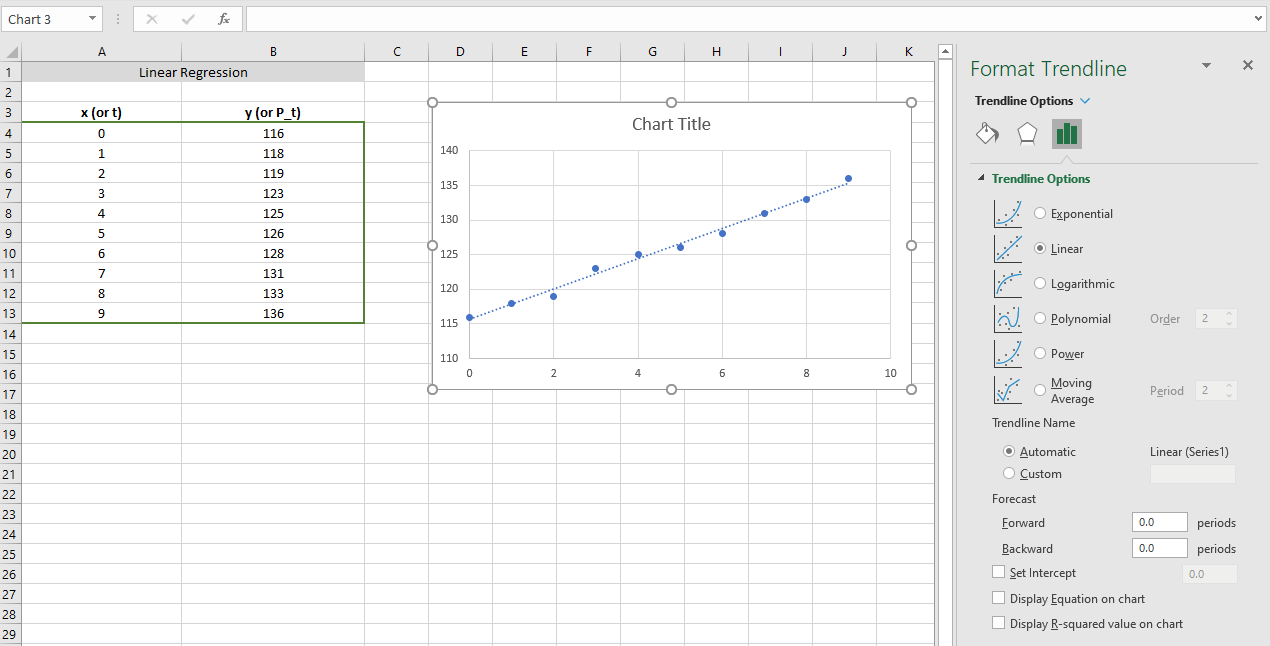
\includegraphics[width=0.6\textwidth]{gmRegressionExcel5}
\end{center}

This leads to the following:

\begin{center}
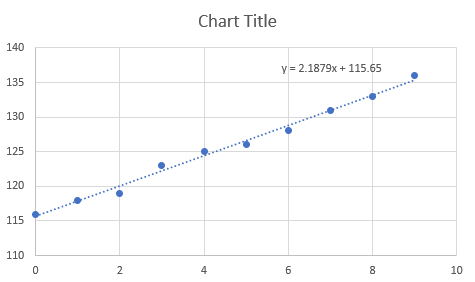
\includegraphics[width=0.6\textwidth]{gmRegressionExcel6}
\end{center}

The equation, as calculated by Excel, is \[P_t = 115.65 + 2.1879t\] which, after rounding, is identical to the one obtained by the calculator (this is no surprise, since they're using the same formulas).

\subsection{When Good Models Go Bad}
When predicting the future with mathematical models, it is crucial to keep in mind that few trends continue indefinitely.

\begin{example}[https://www.youtube.com/watch?v=7_wAlvsCyDc&list=PLfmpjsIzhztutjEb8Pg5OBOlI1p80yVoy&index=3]{A Boy's Height}
Suppose a four year old boy is currently 39 inches tall, and you are told to expect him to grow 2.5 inches a year.\\

We can set up a growth model, with $t=0$ corresponding to 4 years old.
\[P_t = 39 + 2.5t\]

At six years old (when $t=2$), we would expect him to be
\[P_2 = 44 \textrm{ inches tall},\]
but this model eventually breaks down.  Certainly, we shouldn't expect him to grow at the same rate all his life.  If he did, at age 50 he would be
\[P_{46} = 154 \textrm{ inches } = 12.8 \textrm{ feet tall}.\]
\end{example}

Of course, this boy will not grow at a constant rate, but rather experience growth spurts and ultimately stop growing in his early 20s.  But this example also illustrates that we should check our model against common sense.
\vspace{0.5in}

Let's look at another example that illustrates the need for a common sense check.

\begin{example}[https://www.youtube.com/watch?v=3FeV7lvkATI&list=PLfmpjsIzhztutjEb8Pg5OBOlI1p80yVoy&index=4]{Marathon Times}
The table and graph below show the record times for the marathon for men and women from 1965 to 1980.
\begin{center}\marginnote{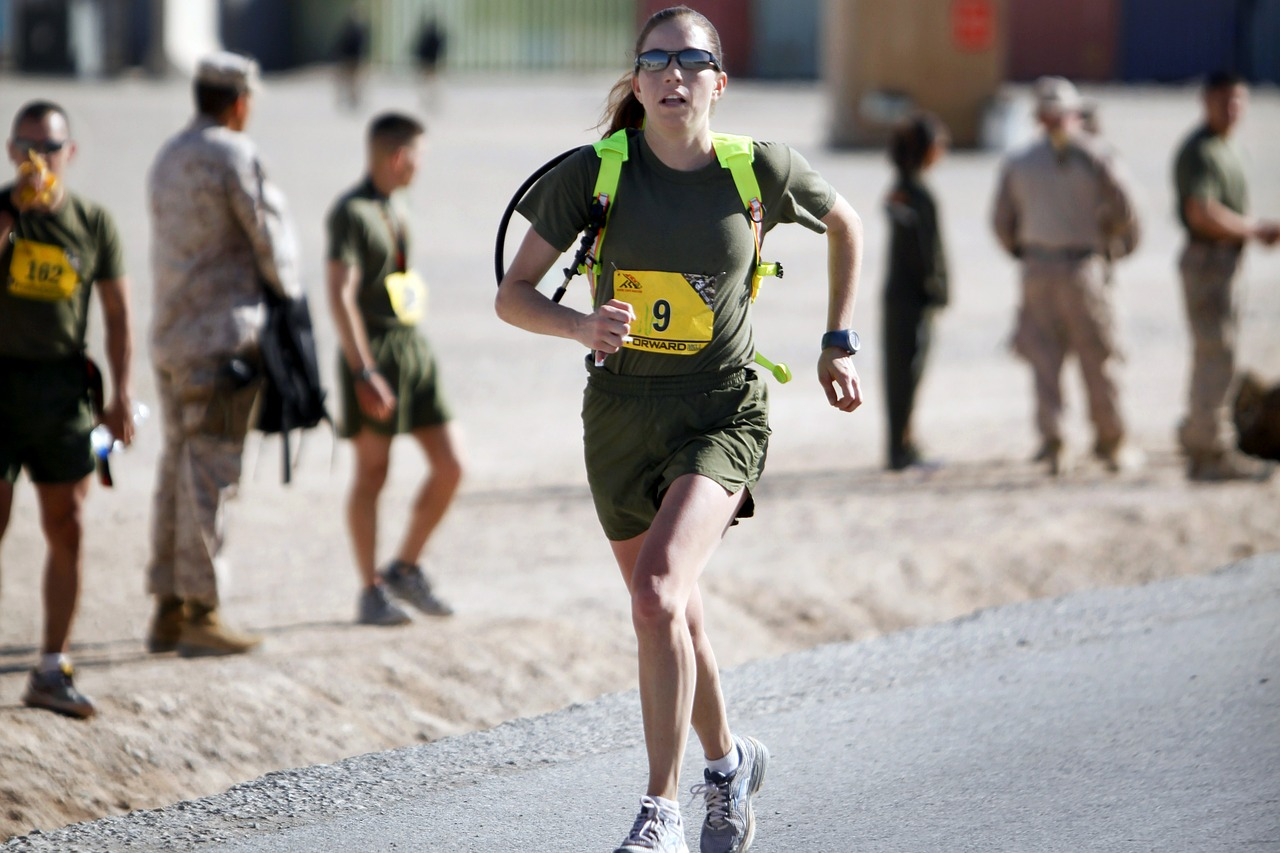
\includegraphics[scale=0.07]{WomanRunner1}}
\begin{tabular}{l | c | c}
\textbf{Year} & \textbf{\color{blue}Men's Times (min)} & \textbf{\color{orange!70!black}Women's Times (min)}\\
\hline
& & \\
1965 & 132 & \\
1966 & & \\
1967 & 129.5 & 195\\
1968 & & \\
1969 & 128.5 & \\
1970 & 129.5 & 183\\
1971 & & 175\\
1972 & & \\
1973 & & 166\\
1974 & 129 & 163\\
1975 & & 158\\
1976 & & \\
1977 & & 155\\
1978 & 129 & 152\\
1979 & & 147\\
1980 & 129 & 145\\
\end{tabular}
\end{center}

\begin{center}
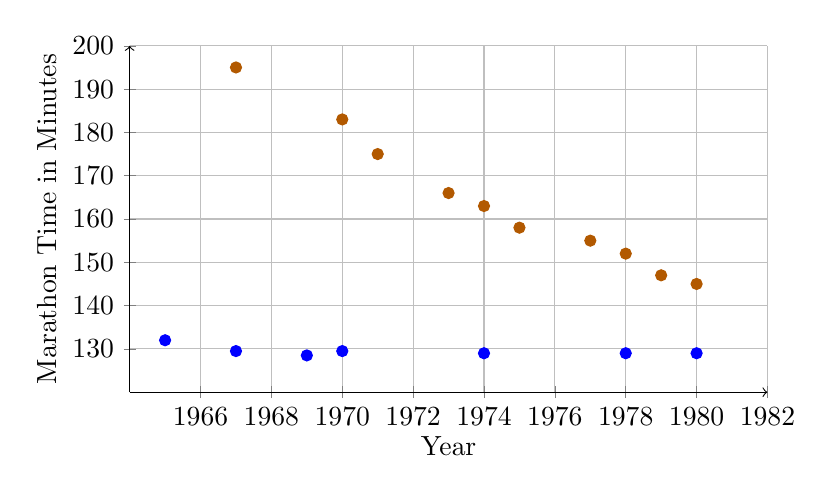
\begin{tikzpicture}
\begin{axis}[
    xmin=0, xmax=18,
    ymin=0, ymax=80,
    axis lines=center,
    axis on top=false,
    domain=0:1,
    x=0.45cm,
    y=0.055cm,
    xtick={0,2,...,18},
    xticklabels={1964,1966,1968,1970,1972,1974,1976,1978,1980,1982},
    ytick={0,10,...,80},
    yticklabels={120,130,140,150,160,170,180,190,200},
    axis lines=middle,
    axis line style={->},
    x label style={at={(axis description cs:0.5,-0.1)},anchor=north},
    y label style={at={(axis description cs:-0.1,.5)},rotate=90,anchor=south},
    xlabel={Year},
    ylabel={Marathon Time in Minutes},
    grid=major
    ]
	\addplot [blue,only marks] table {
	1 12
	3 9.5
	5 8.5
	6 9.5
	10 9
	14 9
	16 9
	};
	\addplot [orange!70!black,only marks] table {
	3 75
	6 63
	7 55
	9 46
	10 43
	11 38
	13 35
	14 32
	15 27
	16 25
	};
\end{axis}
\end{tikzpicture}
\end{center}

From this data, it looks like both sets of data are following a linear trend.  If we use the first and last data points to find the average rate of change for each, we get the following linear models, using 1967 as $t=0$:
\begin{align*}
M_t &= 129.5-0.2t\\
W_t &= 195-3.85t
\end{align*}

According to these two linear models, we would predict that the women's record would beat the men's record by 1985; however, in 1985, the men's record was still 14 minutes faster than the women's.  What happened here?\\

Since women began setting marathon records about 50 years later than men, in the early years their progress was drastic, but eventually slowed down, and the trend was not linear over the long run (wow, what a terrible pun).
\end{example}

It should be clear that this linear trend was misleading, since if we extrapolated this model too far forward, we'd get ridiculous results.  The model predicts, for instance, that women would run the marathon in 1:20:00 in 1997 (a pace of about 20 mph, the speed of a roadrunner or close to the top speed of Usain Bolt at full sprint), or that by 2017 they'd be running it in 2.5 minutes (around 630 mph).

The lesson is simple, and hopefully obvious: linear trends are usually only useful in the short term; few phenomena follow linear trends over the long term.  That is why we'll examine other types of models in the coming sections.  However, keep this in mind, because we'll find that even those more sophisticated models have their limitations, and often they too break down in the long term.